% OCR draft from PDF pages 23-50. Needs cleanup and verification.
\chapter{Introduction}
\label{chap:introduction}

\section{Simulations and Systems}
\label{sec:simulations-and-systems}

A variety of types, levels, and forms of simulation are used in computer and
communication system design. We'll begin with a brief look at some of the terms
used in describing simulations, systems, and simulation languages.

Simulations. The type of simulation which is our subject is called
discrete-event system-level simulation. Discrete-event systems change state at
discrete points in time, as opposed to continuous systems, which change state
over time. (Although not our concern, a variety of fascinating continuous-time
simulation models are used in computer system design to analyze such things as
heat dissipation, ink drop formation for ink jet printers, and the acceleration
profile for voice-coil-driven disk actuators.)

Computer systems are modeled at several levels of detail: circuit-level,
gate-level, register-transfer-level, and system-level. Each level represents a
higher level of abstraction. At the circuit-level, continuous-time simulation is
used to analyze state switching behavior. The components -- transistors,
resistors, etc. -- of a circuit are aggregated into a single element in
gate-level simulation. At the register-transfer-level, sets of gates are
aggregated into elements such as registers, multiplexors, and adders.
System-level simulation begins at a level somewhere above the register-transfer
level. Gate-level, register-transfer-level, and system-level simulation all are
forms of discrete-event simulation. Gate- and register-transfer-level models
are developed to analyze the behavior of the system from a functional
standpoint, and represent the complete system design at different levels of
abstraction. System-level models are developed to analyze the system from a
performance standpoint, and represent only those elements of the system
pertinent to the performance issue of concern.

Determining which elements of the design are to be represented in the
system-level model and the level of abstraction with which these elements are to
be represented is a matter of judgement.

Simulation input data may be generated probabilistically within the simulation
program, or it may be generated externally. In trace-driven simulation,
simulation input is obtained from a trace of actual system execution. Various
kinds of traces are useful in computer performance evaluation: instruction
traces are used to drive pipeline models, address traces to drive cache models,
and I/O traces to drive disk subsystem models. System accounting data has been
used to drive computer system scheduling models. Our discussion deals only with
internally-generated simulation input data; for a discussion of trace-driven
simulation and further references, see Kobayashi [1978] or Ferrari [1978].

A hybrid simulation model combines a discrete-event simulation model and an
analytic (e.g., queueing) model so as to reduce computational time while
preserving model accuracy. (The term also is used to describe a combination of
digital computer and analog computer simulation.) This is an important concept:
we'll return to it in Chapter 3.

Systems. In modeling a system, we need to describe its dynamic composition, the
way it accomplishes work, not just its static structure. The dynamic
composition of a system can be described in terms of activities, processes, and
events [MacDougall 1975].

Performance measures relate to the rate at which systems accomplish work, and
so have time as an independent variable. Work is accomplished through the
execution of activities. An activity is the smallest unit of work in our view
of a system. Since it is a unit of work, every activity has an associated
execution time. A logically-related set of activities constitutes a process.
The execution time of a process is (ignoring concurrency) the sum of the
execution and delay times of its activities. A process may, in turn, be viewed
as an activity of a higher-level process. For example, execution of a program
may be viewed as a process comprising compute and input/output activities;
execution of an input/output activity may be viewed as a process comprising
seek, latency, and data transfer activities. The distinction depends on our
level of view.

Systems are composed of both active and passive entities; we can view the
work-performing facilities of a system as simple passive objects which assume
one of two states -- busy or idle -- as the result of actions of activities.
Such objects also are decomposable. At one level of view, a CPU may be
represented as a single passive entity made busy or idle by compute activities.
At a more detailed view, compute activities can be decomposed into instruction
execution processes comprising instruction fetch, operand fetch, execute, and
result store activities. Correspondingly, the CPU is decomposed into
instruction fetch, cache, pipeline, execution, and mainstore units. Also, a
passive entity at one level of view may decompose into a combination of active
and passive entities at another level of view.

The initiation of activities is triggered by events. An event is a change of
state of some system entity, active or passive; this change of state results
from the action of an activity. The termination of an activity is an event.
The initiation of an activity is distinguished from the start of its execution;
for example, termination of a task's compute activity may initiate its
input/output activity, but execution of the latter cannot begin until the disk
is free. An activity whose execution is delayed because the requisite
conditions do not exist can be viewed as waiting for the event(s) which will
give rise to those conditions. Activity termination events are local to the
process to which the activity belongs; events representing a state change in a
passive system entity may have a wider scope.

These entities -- activities, processes, and events -- are the constructs used
to describe the dynamic behavior of discrete systems and on which simulation
languages for these systems are based. A system is viewed dynamically as a
collection of interacting processes, with the interactions controlled and
coordinated by the occurrence of events. This process view is a hierarchical
one; a system is described at a given level of abstraction by a set of process
descriptions, each specifying the activities of that process. This description
can be expanded into a lower level of abstraction by decomposing activities
into processes; description of these processes, together with those of the
previous level, form the expanded description of the system. This hierarchical
view can substantially ease the task of model construction for complex systems.

A hierarchical approach (sometimes different in nature) is important in other
kinds of modeling. Lazowska et al [1984] describe how complex queueing network
models are solved by decomposing the network into a set of submodels,
evaluating each submodel separately, and combining these individual solutions
in a higher-level model to obtain a solution for the whole system. MacDougall
[1984] applies decomposition at the instruction level to the evaluation of
pipelined processors.

Simulation languages. Simulation languages are classified as activity-oriented,
event-oriented, or process-oriented, based on the procedural organization of
simulation programs written in that language. A procedural section of a
simulation program may describe an activity, an event, or a process, depending
on the language used. Correspondingly, a model of a system is viewed as a set
of activity descriptions, event descriptions, or process descriptions; each
language tends to impose a particular view of the system on the modeler.

Almost all present-day simulation languages are event- or process-oriented.
Process-oriented languages such as ASPOL [MacDougall 1975], CSIM [Schwetman
1986], or SIMULA [Birtwhistle et al 1973] are strongly recommended for
implementing large-scale simulation models. Simulation programs written in
these languages can be constructed as straightforward descriptions of actual
system operation. This similitude of model and system makes it much easier to
insure that the model is a valid representation of the system, particularly in
a development environment where the system design is undergoing constant
change. The hierarchical nature of process-oriented languages also is
important in the development environment.

Event-oriented simulation languages such as smpl are best suited to small- and
medium-scale models. They tend to impose a single-level, global view of the
system on the modeler. There is a tendency to collect actions of logically
unrelated activities in a single event routine; as a consequence, the model can
lose all identity with the structure of the system and become difficult to
modify. This problem can be minimized by careful structuring of the model --
taking a process-oriented view of the system and organizing the model
accordingly.

\section{Representing Work}
\label{sec:representing-work}

Developing a model involves two tasks: developing a representation of the
system, and developing a representation of the work done by the system. These
are inter-related: the level of abstraction at which work is represented must
correspond to that at which the system is represented. Before building a very
detailed model of a system, we should ask two questions. Do we really need to
work at this level of detail to solve the problem? Do we have data to represent
work at this level?

The task of describing the work performed by a system is called workload
characterization; it is a key step in several areas of performance evaluation,
including simulation modeling, analytic modeling, and benchmarking. Ferrari
[1978] discusses system-level, source-program-level, and instruction-level
workload characterization, and is the best of our referenced texts in this
subject area. In this section we will look at some considerations in
representing work in a simulation model.

\paragraph{Variability.}
Most of the problems we want to analyze center around contention for system
resources; this contention causes work to be queued for or blocked from
execution, and system performance may suffer as a result. Contention arises
because of variability in some aspect of system behavior: in the way work
arrives at the system, in its execution time, or both. Suppose tasks arrive at a
system at an average interval of 10 units, and each task requires an average
service time of 6 time units. If there is no variability in inter-arrival or
service times, so that they are the same for all tasks, no queueing delays
occur, since every arriving task will find the system idle. If there is
variability in either or both of these times, then delays may occur; their
magnitude depends on the amount of variability and on the extent to which
these times may be correlated. In describing the work of a system, then, we
need to consider the distributions of the associated variables, not just their
mean values. We also need to examine behavior patterns to determine if and how
these variables are correlated.

\paragraph{Choosing a distribution.}
Determining what distribution to use to represent a model variable is one of
the most difficult aspects of simulation modeling. When the system being
modeled exists, we may be able to measure it, obtain actual distributions, and
use these in our model. There are two ways to do this; we can tabulate values
of the distribution and do a table look-up to obtain a sample value, or we can
fit a theoretical distribution to the actual distribution and use an algorithm
to generate a sample value. Common probability distributions, their
parameters, and the estimation of parameters from data are discussed in Banks
and Carson [1984], Bratley et al [1983], and Law and Kelton [1982]. The
discussion in Law and Kelton is the most comprehensive of the three. This
subject also is covered in most applications-oriented statistics texts.

At one time, fitting a distribution to data often involved transforming the
data into various forms and plotting it on probability paper appropriate to the
distribution of interest. Computer programs now are available which
substantially reduce the time and effort required. An example is UNIFIT [Law
and Vincent 1983], which permits a variety of data transformations, fits up to
nine different distributions simultaneously using any of several different
goodness-of-fit tests, and provides a number of graphics displays of the
results.

If we're modeling a new design and there is no system to be measured:
what then? One possibility is to adapt a distribution measured on some existing
system -- assume the shape of the distribution will be similar on the new
system and adjust the values to reflect system differences. Suppose we are
modeling a new computer system and need to specify the distribution of CPU
execution intervals; if measurements of this distribution on the current system
are available, we can rationalize that the number of instructions executed per
interval will be about the same on both systems, and adjust the interval by the
ratio of instruction execution rates for the two systems. This may be our best
course, but it shouldn't be followed blindly: we need to examine carefully our
assumption that the distributional characteristics of the work won't change
when the system changes.

We frequently will find ourselves in a situation where we have very little data
and no idea what the actual distribution of the data looks like. In order to
proceed, we'll have to do some guessing (and, when the model is complete, do
some experimentation to determine how sensitive the results are to our
guesswork). Suppose the variable of interest is the processing time at some
facility. We first try to specify an interval bounded by the best-case and
worst-case times a and b. Next, we try to visualize how times may be skewed in
this interval. One way to do this is to quarter the interval and guess what
proportion of times are likely to fall in each quarter, or quartile. We can
then fit a distribution with approximately the same quartile proportions. (Our
understanding of the nature of the process may suggest a different division.)
If we have no reason to believe that times are more likely to fall in one
quartile than another, the best we can do is assume that processing times are
uniformly distributed in [a,b]. If we can estimate the mode, as well as upper
and lower bounds, we can use a triangular distribution (see Law and Kelton
[1982], p205, or Banks and Carson [1984], p157).

\paragraph{The exponential distribution.}
The most important distribution in the analysis of queueing systems is the
negative exponential or, simply, the exponential distribution. When we talk
about random arrivals or random service, we mean that the inter-arrival times
or the service times are exponentially distributed. Equivalently, because of
the relationship between the Poisson and exponential distributions, we might
talk about Poisson arrivals or service (if the number of events occurring in an
interval is Poisson-distributed, the time between events is exponentially
distributed).

An important property of the Poisson process is that it is memoryless; the
probability of an arrival in interval t depends only on the duration of t, and
not on when the previous arrival occurred. Equivalently, for Poisson service,
the probability that service completes in an interval s is independent of when
service started. This memoryless property is the key to obtaining analytic
solutions for many queueing problems; consequently, there exists considerable
rationalization for the exponential assumption ("there is no virtue like
necessity").

Another useful property of the Poisson process is that the superposition of
Poisson processes is itself a Poisson process. Suppose we are modeling a
transaction processing system with a number of terminals: if transactions are
generated at each terminal according to a Poisson process, then the composite
transaction stream seen by the system also is a Poisson process (see
[Kobayashi 1978]). In fact, the individual transaction sources don't
necessarily have to be Poisson: if the sources are independent and no one
source dominates (and certain other conditions hold), the superposition of the
individual transaction streams approaches a Poisson process as the number of
sources increases. Inter-arrival times, then, frequently are assumed to be
exponentially distributed; we'll probably make the same assumption whenever we
can't discern any pattern to the arrival process.

Other important distributions include the Erlang and hyperexponential
distributions, both of which are related to the exponential distribution. A
k-Erlang distribution can be represented as the sum of k identical
exponentially-distributed random variables. A k-stage hyperexponential
distribution is a mixture of k different exponential distributions. These are
discussed in the referenced simulation and performance evaluation texts.

\paragraph{Sampling from distributions.}
A particular value of a model variable is determined by generating a random
sample from the distribution specified for that variable. A particular sample
value usually is called a random variate.\footnote{The term "pseudo-random"
sometimes is used to emphasize that the underlying process actually is
deterministic.} There are numerous techniques for generating these samples, all
of which employ a uniform random number generator. A uniform random number
generator is a numerical algorithm which produces a deterministic sequence of
values distributed between 0 and 1. There are a number of desirable
characteristics for this sequence: uniformity, independence, long period
(length of the sequence before it begins to repeat), etc. The design and
testing of random number generators is discussed at length in the referenced
texts on simulation; also, see Knuth [1981]. A word of caution: don't use the
random number generator in your system's math function library until you've
verified that it is a reasonable algorithm.

The generation of random variates from a variety of distributions also is
discussed in our simulation texts. For a variety of common distributions,
Fortran implementations can be found in Bratley et al [1983], and outlines of
sampling algorithms in Fishman [1978]. Hastings and Peacock [1974] give brief
descriptions of generators for a number of distributions. We'll consider two
examples of variate generators here: one using an empirical distribution, and
one using a theoretical distribution.

Suppose modeling task execution in a microcomputer system simulation requires
generating sample values of the lengths of the files associated with each task.
We'll assume that measurements of system operation have produced the file
length distribution shown in Figure 1.1. This is a discrete distribution: the
possible values of the variate are 1, 2, ..., 10. To generate a random file
length, we first convert the distribution to cumulative form, obtaining the
proportions P[I<L] of files whose lengths are equal to or less than L. Next, we
generate a random number r and find the value of L for which P[I<L-1] < r <
P[I<L]; that value is our sample value.

This process is illustrated in Figure 1.2. The cumulative distribution of file
lengths is plotted on the right; the vertical bar to the left of the plot shows
the values of the cumulative proportions. Imagine a set of random numbers are
generated; the values of these numbers would fall uniformly across the bar; a
value falling between the marks corresponding to P[I<L-1] and P[I<L] generates
a sample value of L. If we generate a large enough set of numbers, the
proportion of these falling in this interval will approach a value P[I<L] -
P[I<L-1]; this value is the proportion of files of length L.

\begin{figure}[htbp]
  \centering
  % Figure 1.1 (left): boxed table of file-length distribution.
  \begin{minipage}{0.38\textwidth}
    \centering
    \renewcommand{\arraystretch}{0.95}
    \fbox{%
      \begin{tabular}{c c}
        \textbf{length in} & \textbf{proportion} \\
        \underline{\textbf{tracks}} & \underline{\textbf{of files}} \\
        1  & .060 \\
        2  & .170 \\
        3  & .238 \\
        4  & .223 \\
        5  & .156 \\
        6  & .087 \\
        7  & .040 \\
        8  & .016 \\
        9  & .007 \\
        10 & .003 \\
      \end{tabular}%
    }
  \end{minipage}\hfill
  % Figure 1.1 (right): histogram with hatched bars.
  \begin{minipage}{0.52\textwidth}
    \centering
    \begin{tikzpicture}
      \begin{axis}[
        width=\textwidth,
        height=0.72\textwidth,
        ymin=0,
        ymax=0.25,
        xmin=0.3,
        xmax=10.7,
        ytick={.00,.05,.10,.15,.20,.25},
        yticklabels={\axisfont .00,\axisfont .05,\axisfont .10,\axisfont .15,\axisfont .20,\axisfont .25},
        xtick={1,2,3,4,5,6,7,8,9,10},
        xticklabels={\axisfont 1,\axisfont 2,\axisfont 3,\axisfont 4,\axisfont 5,\axisfont 6,\axisfont 7,\axisfont 8,\axisfont 9,\axisfont 10},
        tick label style={font=\axisfont\small,/pgf/number format/assume math mode=false},
        xticklabel style={font=\axisfont\small,/pgf/number format/assume math mode=false},
        yticklabel style={font=\axisfont\small,/pgf/number format/fixed,/pgf/number format/assume math mode=false},
        axis lines=box,
        axis line style={line width=2.2pt},
        tick style={black,line width=1pt},
        major tick length=6pt,
        minor tick length=3pt,
        minor y tick num=1,
        tick align=outside,
        xtick pos=left,
        ytick pos=left,
        enlargelimits=false,
        ymajorgrids=false,
        xmajorgrids=false,
      ]
        % Figure 1.1 histogram: horizontal dashed guides at selected heights.
        \addplot[black!50, dashed, line width=0.6pt, forget plot] coordinates {(0.5,0.060) (10.5,0.060)};
        \addplot[black!50, dashed, line width=0.6pt, forget plot] coordinates {(0.5,0.170) (10.5,0.170)};
        \addplot[black!50, dashed, line width=0.6pt, forget plot] coordinates {(0.5,0.238) (10.5,0.238)};
        \addplot[black!50, dashed, line width=0.6pt, forget plot] coordinates {(0.5,0.223) (10.5,0.223)};
        \addplot[black!50, dashed, line width=0.6pt, forget plot] coordinates {(0.5,0.156) (10.5,0.156)};
        \addplot[black!50, dashed, line width=0.6pt, forget plot] coordinates {(0.5,0.087) (10.5,0.087)};
        \addplot[
          ybar,
          bar width=0.081\textwidth,
          fill=white,
          draw=black,
          pattern={Lines[angle=45,distance=3pt,line width=1.5pt]},
          line width=3pt
        ]
          coordinates {
            (1,.060) (2,.170) (3,.238) (4,.223) (5,.156)
            (6,.087) (7,.040) (8,.016) (9,.007) (10,.003)
          };
      \end{axis}
    \end{tikzpicture}
  \end{minipage}
  \caption{Distribution of File Lengths}
  \label{fig:file-lengths}
\end{figure}

\begin{figure}[htbp]
  \centering
  % Figure 1.2 (left): uniform random variate scale + arrow.
  \begin{minipage}{0.3\textwidth}
    \hspace*{0.6cm}
    \pgfmathsetlengthmacro{\figtwoheight}{0.72\textwidth}
    \begin{tikzpicture}[x=1cm,y=\figtwoheight/5]
      \draw[->,line width=1pt] (0,0) -- (0,5);
      \foreach \y in {0,1,2,3,4} {
        \draw[line width=0.8pt] (-0.15,\y) -- (0.15,\y);
      }
      \draw[line width=0.8pt] (-0.30,0) -- (0.30,0);
      \draw[line width=0.8pt] (-0.30,5) -- (0.30,5);
      \node[rotate=90] at (-1.0,2.5) {random variate uniform in [0, 1]};
      \draw[-{Latex[length=3mm]},line width=0.8pt] (0.7,2.5) -- (1.8,2.5);
    \end{tikzpicture}
  \end{minipage}\hspace*{0.4cm}
  % Figure 1.2 (right): cumulative sampling box.
  \begin{minipage}{0.50\textwidth}
    \centering
    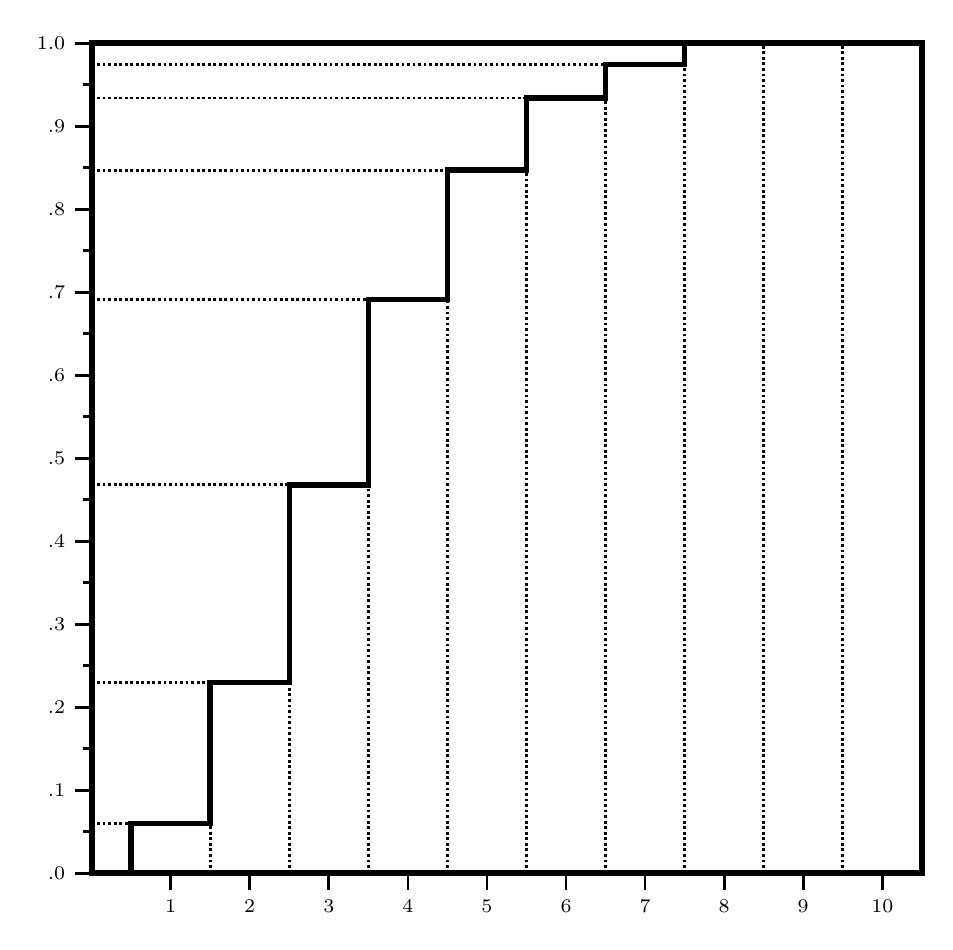
\begin{tikzpicture}
      \begin{axis}[
        width=1\textwidth,
        height=1\textwidth,
        ymin=0,
        ymax=1.0,
        xmin=0.5,
        xmax=11.0,
        ytick={0.0,0.1,0.2,0.3,0.4,0.5,0.6,0.7,0.8,0.9,1.0},
        yticklabels={\axisfont .0,\axisfont .1,\axisfont .2,\axisfont .3,\axisfont .4,\axisfont .5,\axisfont .6,\axisfont .7,\axisfont .8,\axisfont .9,\axisfont 1.0},
        xtick={1.5,2.5,3.5,4.5,5.5,6.5,7.5,8.5,9.5,10.5},
        xticklabels={\axisfont 1,\axisfont 2,\axisfont 3,\axisfont 4,\axisfont 5,\axisfont 6,\axisfont 7,\axisfont 8,\axisfont 9,\axisfont 10},
        axis lines=box,
        axis line style={line width=2.2pt},
        tick style={black,line width=1pt},
        major tick length=6pt,
        minor tick length=3pt,
        minor y tick num=1,
        tick align=outside,
        xtick pos=left,
        ytick pos=left,
        tick label style={font=\axisfont\scriptsize,/pgf/number format/assume math mode=false},
        xticklabel style={font=\axisfont\scriptsize,/pgf/number format/assume math mode=false},
        yticklabel style={font=\axisfont\scriptsize,/pgf/number format/assume math mode=false},
        enlargelimits=false,
        xmajorgrids=false,
        ymajorgrids=false,
        grid style={dotted, line width=0.6pt},
      ]
        % Figure 1.2 box: short horizontal dotted connectors from y-axis.
        \addplot[densely dotted, line width=1pt, forget plot] coordinates {(0.5,0.060) (1.0,0.060)};
        \addplot[densely dotted, line width=1pt, forget plot] coordinates {(0.5,0.230) (2.0,0.230)};
        \addplot[densely dotted, line width=1pt, forget plot] coordinates {(0.5,0.468) (3.0,0.468)};
        \addplot[densely dotted, line width=1pt, forget plot] coordinates {(0.5,0.691) (4.0,0.691)};
        \addplot[densely dotted, line width=1pt, forget plot] coordinates {(0.5,0.847) (5.0,0.847)};
        \addplot[densely dotted, line width=1pt, forget plot] coordinates {(0.5,0.934) (6.0,0.934)};
        \addplot[densely dotted, line width=1pt, forget plot] coordinates {(0.5,0.974) (7.0,0.974)};
        % Figure 1.2 box: step function (cumulative).
        \addplot[const plot,line width=2pt]
          coordinates {
            (0,0)
            (1,0.060)
            (2,0.230)
            (3,0.468)
            (4,0.691)
            (5,0.847)
            (6,0.934)
            (7,0.974)
            (8,1.000)
            (9,1.000)
            (10,1.000)
          };
        % Figure 1.2 box: vertical dotted guides at each integer.
        \addplot[densely dotted,line width=1pt] coordinates {(1,0) (1,0.060)};
        \addplot[densely dotted,line width=1pt] coordinates {(2,0) (2,0.060)};
        \addplot[densely dotted,line width=1pt] coordinates {(3,0) (3,0.230)};
        \addplot[densely dotted,line width=1pt] coordinates {(4,0) (4,0.468)};
        \addplot[densely dotted,line width=1pt] coordinates {(5,0) (5,0.691)};
        \addplot[densely dotted,line width=1pt] coordinates {(6,0) (6,0.847)};
        \addplot[densely dotted,line width=1pt] coordinates {(7,0) (7,0.934)};
        \addplot[densely dotted,line width=1pt] coordinates {(8,0) (8,1.000)};
        \addplot[densely dotted,line width=1pt] coordinates {(9,0) (9,1.000)};
        \addplot[densely dotted,line width=1pt] coordinates {(10,0) (10,1.000)};
      \end{axis}
    \end{tikzpicture}
  \end{minipage}
  \caption{Sampling the File Length Distribution}
  \label{fig:sample-file-length}
\end{figure}

A C function flength() to generate a random file length might be written as
follows. (OCR needs verification.)

\begin{verbatim}
flength ()
{
static double p[10]=
.060, .230, .468, .691, .847, .934, .974, .990, .997, 1.0;
int i = 0;
double r;
r = ranf ();
while (r > p[i]) i++;
return (i+1);
}
\end{verbatim}

There are several points about this process worth noting. First, in this
example, we can directly compute the sample value from the index to array p[]
(by adding 1). Sometimes we can do this, and sometimes we'll have to define an
array of sample values and use the index to obtain a value from the array.
Second, suppose at some place in our model we need to randomly select 1 of n
alternatives, and each alternative has a different probability associated with
it. The random selection function would look very much like the function above,
except it would return alternative numbers rather than file lengths (but if
alternatives are equiprobable, we'd probably just use an expression such as
"1+n*ranf()" to pick one).

A similar approach can be used to generate sample values from continuous
distributions. For example, suppose measurements of disk seek times give the
proportions p(ti-1,ti) of seek times falling in intervals ti-1, ti. To implement
our sampling function, we define two arrays, one containing the interval
endpoints t0, t1, t2, ... , the other containing the cumulative proportions 0,
P[t<t1], P[t<t2], ... . To generate a sample value, we generate a random number
r and use it to find the entry in the array for which P[t<ti-1] < r < P[t<ti].
The sample seek time is determined by interpolation between the corresponding
entries in the seek time interval endpoint array. The sample-generating
statements might look like this (OCR needs verification):

\begin{verbatim}
r = ranf ();
while (r > p[i]) i++;
t = t[i-1] + (t[i]-t[i-1]) * (r - p[i-1]) / (p[i] - p[i-1]);
\end{verbatim}

There are several things we can do (in addition to coding changes) to make
sample generation more efficient. If there are more than a few entries, we can
use a binary, rather than a linear, search of p[]. The intervals used to divide
the distribution don't have to be the same width; we can use short intervals
where the distribution changes shape rapidly and long intervals where the rate
of change is slow to optimize the number of entries.

In both examples, we tabulated the cumulative distribution function p = F(x),
generated a random value of p, and used the tabulation to obtain the
corresponding value of x; in effect, we generated values of the inverse
function \ensuremath{x = F^{-1}(p)}. In some cases, it is possible to determine directly the
inverse of the distribution function of a theoretical distribution. For
example, suppose inter-arrival times are exponentially distributed with mean T;
the probability that an arrival time x is equal to or less than t is given by

\begin{align}
\Pr[x<t] &= 1 - e^{-t/T} \tag{1.1}\label{eq:exp-cdf}\\
t &= -T \ln(1-r) \tag{1.2}\\
t &= -T \ln r \tag{1.3}
\end{align}

where ln(x) denotes the natural logarithm of x. Since r is a random variate
uniformly distributed in [0,1], 1-r is identically distributed; therefore, we
can rewrite (1.2) as (1.3). We can use (1.3) to write a C function to generate
sample values from the exponential distribution. The following function is one
of the smpl random variate generation functions.

\begin{verbatim}
double expntl (t)
double t;
{
  double ranf();
  return (-t*log(ranf()));
}
\end{verbatim}

Unfortunately, direct inversion of the distribution function is possible only
for a few distributions; other techniques for generating variates frequently
are needed. For most of our simulation work, we'll manage with the smpl
sampling functions supplemented by those presented in our simulation texts.
Nevertheless, familiarity with random variate generation techniques is useful;
among other things, it provides ideas for incorporating analytic results in our
simulation models. Of course, if pressed, we can tabulate values of the
distribution function for any discrete or continuous distribution, and generate
samples as we did in our earlier examples.

There are a few things to keep in mind when sampling theoretical distributions.
First, do the values returned by your random number generator include 0? If so,
you will have to be sure that your sampling functions don't attempt to take the
logarithm of a zero value. Theoretical distributions may have tails extending
to infinity on one or both sides, and samples may need to be clipped. Most
variables in computer system simulations don't have negative values: when
sampling from the normal distribution, inspect samples and discard negative
values. Generators for distributions such as the exponential distribution can
return very large values; you may want to truncate the sample distribution to
reflect the maximum value realizable in the actual system. The mean value of
samples from (for example) a truncated exponential distribution may differ from
the exponential distribution's mean unless the latter is adjusted. Section 6.8
discusses computation of an adjusted mean for a truncated exponential
distribution.

\paragraph{Correlation.}
There are two kinds of correlation that may need be represented in a model. One
is autocorrelation, where successive values from a distribution are not
independent but reflect some underlying relationship. This is a difficult
subject in terms of both workload characterization and model representation.
Fishman [1978] describes two ways of generating autocorrelated sequences.

The second kind of correlation is that between jointly-distributed variables:
variables from different distributions representing different aspects of work.
For example we would expect compiler execution times and compiler input file
lengths to be correlated, in which case a functional relationship could be
obtained via regression analysis of measurement data. To generate attributes
of a particular compilation in a simulation model, we could generate a sample
input file length and use its value to compute a sample compilation time.
Modeling such relationships mostly involves common-sense tradeoffs between
model accuracy and complexity. Developers of synthetic workloads face similar
problems and have developed sampling approaches: see, for example, Hughes
[1984], and Sreenivasan and Kleinman [1974].

\section{A Simple Queueing Simulation}
\label{sec:simple-queueing-sim}

This section presents a simulation model of a simple queueing system written in
C without the use of smpl. We'll review some of the performance measures of
interest in queueing system analysis and discuss basic simulation operations.
First, let's look at how queueing systems are described.

Queueing notation. A standard notation (called Kendall notation after its
originator) is used to describe queueing systems with a single queue and one or
more parallel servers. This notation is commonly used in the literature, so
it's useful to be familiar with it. Using this notation, a queueing system is
described by a descriptor of the form A/S/c/k/m, where A represents the
inter-arrival time distribution, S represents the service time distribution, c
is the number of servers, k is the maximum number of customers allowed in the
system, and m is the number of customers available at the source.\footnote{Use
of the term ``customer'' to describe a system's work-bearing entities and
``server'' to describe its work-performing entities is traditional. Also,
``queueing system'' frequently is shortened to ``queue''.} Among the symbols
commonly used to describe distributions are:

\begin{verbatim}
D   constant inter-arrival or service time
M   exponential distribution
Ek  k-Erlang distribution
Hk  k-stage hyperexponential distribution
G   general (arbitrary) distribution
\end{verbatim}

When the customer population is assumed to be infinite, m usually is omitted;
similarly, when the system capacity is assumed to be infinite, k is omitted.
The queueing discipline may be appended to the descriptor; if not, it can be
assumed to be first-in, first-out. Using this notation, a queueing system with
exponential inter-arrival times, constant service times, and a single server is
described as an M/D/1 queue; a system with exponential inter-arrival times,
general service times, 2 servers, and a queue capacity of k customers is
described as an M/G/2/k queue.

The queueing system model. The system to be simulated is the single server
queueing system shown in Figure 1.3. Work for the system comes from an
infinite population of customers; the inter-arrival times of customers at the
system are exponentially distributed with mean Ta. On arrival, a customer
begins service if the server is free or joins the queue if the server is busy.
The queue capacity is unlimited, and the queueing discipline is first-in,
first-out; whenever one customer completes service, the next customer to begin
service is the one at the head of the queue. Service times are exponentially
distributed with mean Ts. (This, then, is an M/M/1 queue.)

\begin{figure}[htbp]
  \centering
  \fbox{\parbox{0.8\textwidth}{TODO: Figure 1.3. A Single Server Queueing System}}
  \caption{A Single Server Queueing System}
\end{figure}

The C program of Figure 1.4 is a simulation model of this system, and is about
as simple as we can get. It uses the expntl() function discussed in the last
section to generate inter-arrival and service times. The mean inter-arrival
time Ta is 200 time units, the mean service time Ts is 100 time units, and the
period of time to be simulated, te, is 200000 time units (so we would expect to
simulate approximately 1000 arrivals). time represents simulated time, and n
is the number of customers in the system at any point in time. There are two
events: event 1 represents arrivals and event 2 represents service completions.
Associated with events 1 and 2 are the event occurrence times t1 and t2; these
are the times at which the next instance of the event will occur.

The model advances through time in variable intervals, rather than constant
"ticks". At any instant, t1 is the time of the next arrival and t2 is the time
of the next completion; to determine which event occurs next, these times are
compared. If t1<t2, then the next event is an arrival. time is advanced to the
arrival time, the count of the number of customers in the system is incremented,
and the time at which the next arrival is to occur is computed. If the system
was empty when this customer arrived, the time at which its service will
complete is computed. If t1>t2, then the next event is a service completion:
time is advanced to the completion time and the number of customers in the
system is decremented. If there are still customers in the system after this
completion, then the time of the next service completion is computed. (This
implicitly represents dequeueing of the customer at the head of the queue and
the start of its service.) If the current completion empties the system, t2 is
set to te to insure that the next event to occur will be an arrival; note that
this also was done during initialization to insure that the first event would
be an arrival.

\begin{figure}[htbp]
  \centering
  \begin{minipage}{0.9\textwidth}
    \begin{verbatim}
main ()
{
double Ta=200.0,Ts=100.0,te=200000.0,t1,t2,time;
double expntl();
int n;
n=0; t1=0.0; t2=te; time=0.0;
while (time<te)
{
if (t1<t2)
{ /* event 1: arrival */
time=t1; n++; t1=time+expntl(Ta);
if (n==1) t2=time+expntl(Ts);
}
else
{ /* event 2: completion */
time=t2; n--;
if (n>0) t2=time+expntl(Ts); else t2=te;
}
}
}
    \end{verbatim}
  \end{minipage}
  \caption{Queueing System Simulation Model}
\end{figure}

Figure 1.5 graphically illustrates the behavior of the simulated system.
Suppose we observe the system for a period of 600 time units, during which
customers arrive at intervals (i.e., inter-arrival times) of 20, 30, 25, 65, 80,
and 80 time units. The service times of these customers are, respectively, 80,
150, 90, 60, 80, and 90 time units. Figure 1.5(a) shows the sequence of
arrivals, waiting times, and service times in the period; Figure 1.5(b) shows
the corresponding changes in the number of customers in the system. If we
manually step through the simulation program using the above inter-arrival and
service times, we can see how the model generates this behavior.

\begin{figure}[htbp]
  \centering
  \fbox{\parbox{0.8\textwidth}{TODO: Figure 1.5. Queueing System Behavior}}
  \caption{Queueing System Behavior}
\end{figure}

\section{Performance Measures}
\label{sec:performance-measures}

While the program of Figure 1.4 may successfully model the behavior of an M/M/1
queueing system, it isn't of much use until we add instrumentation to collect
the performance measures of interest to us. We can collect just about
anything; mostly we'll be interested in mean values, but on occasion we may
want distributions as well. We'll begin this section with a look at certain
fundamental mean value performance measures and their relationships. Because
these relationships apply widely and hold under very general conditions, some
have come to be called laws.

Suppose we observe the system for a period of time T and measure the number of
arrivals, A, and the number of completions, C. We then can compute the arrival
rate and the throughput rate:

\begin{align}
A &= A/T \tag{1.4}\\
X &= C/T \tag{1.5}
\end{align}

In measuring a real or simulated system, there may be customers in the system
queued for or receiving service both at the start and at the end of the
observation period.
However, if the period is sufficiently long, the number of arrivals observed
should be approximately equal to the number of completions (C = A), in which
case we can assume A = X. This assumption is called the flow balance
assumption: the flow of work out of the system is balanced by the flow of work
into it. When we make this assumption, we only need to count arrivals or
completions, whichever is easier, not both.

Suppose we also measure the mean server busy time, B. Now we can compute the
server utilization and the mean service time per customer:

\begin{align}
U &= B/T \tag{1.6}\\
T_s &= B/C \tag{1.7}
\end{align}

Utilization Law. Through simple algebra, we can combine (1.5), (1.6), and (1.7)
to obtain the Utilization Law:

\begin{align}
U &= X T_s \tag{1.8}\\
U &= A T_s \tag{1.9}
\end{align}

In words, the utilization of a server is the product of its
throughput rate and the average service time per customer.

Little's Law. Let L be the average number of customers in the system during
the observation period, and let W be the average time these customers spend in
the system. Define \ensuremath{w_i} as the time spent in the system by the ith customer:
then \ensuremath{W = \sum w_i / C}. Look back at Figure 1.5(b) for a moment; this is a graph
of the number of customers in the system versus time. The average number of
customers in the system is the average height of the graph; this is equal to
the area under the graph divided by the length of the observation period. Each
customer, while in the system, contributes one unit of height to the graph, and
so contributes 1 x wi to the area under the graph. The total area is the sum
of the contributions of the C customers completing service during the
observation period, which is equal to W C. The average number in the system is
this area divided by the observation time: \ensuremath{L = W C / T}. Since, from (1.5),
\ensuremath{C/T = X}, we can write

\begin{align}
L &= X W \tag{1.10}\\
L &= A W \tag{1.11}
\end{align}

In words, the average number of customers in the system is the product of the
system's throughput rate and the average time a customer spends in the system.

The preceding paragraph gave an informal derivation of Little's Law, named for
J. D. C. Little, who presented the first formal proof [Little 1961]. This law
is one of the most important results in queueing theory (the mnemonic of "law"
for L = AW makes it easy to remember). It doesn't depend on the form of the
inter-arrival or service time distributions or on the queue discipline. Little's
Law can be applied at various levels of a system and in various ways at a given
level. For example, let Lq be the average number of customers queued in the
system (not receiving service), and let \ensuremath{W_q} be the mean queueing time. We can
use the same approach as before to show that

\begin{equation}
L_q = A W_q \tag{1.12}
\end{equation}

Note that \ensuremath{L = L_q + U} and \ensuremath{W = W_q + T_s}. We can consider the Utilization Law to be another
application of Little's Law by viewing U as the average number of customers
receiving service.\footnote{In queueing theory literature, the time a customer
spends in the system -- including service time -- usually is called "waiting
time". (This isn't intuitive to the designer, who separates working time and
waiting time.) Similarly, the term "queue length" is used to describe the
number of customers in the system, including those in service. (Always read the
definition of terms carefully.) We'll call the time a customer spends in the
system its system residence time or its response time, and the time it spends
in the queue (not receiving service) its queueing time.}

Response Time Law. This law commonly is stated in the context of a timesharing
system. Let N be the number of terminals in the system, let Z and R be,
respectively the mean think time and mean response time at a terminal, and let
X be the system throughput. Then

\begin{equation}
R = (N/X) - Z \tag{1.13}
\end{equation}

An example of the use
of this law in a different context is given in Section 5.3.

Let's apply some of these relationships to the queueing system whose behavior
is represented in Figure 1.5. There are C = 6 completions in the observation
period of T = 600 time units. (Arrival, service start, and service completion
times can be obtained by reference to the event times along the time axis of
Figure 1.5(b)).

\begin{align*}
\text{throughput:} &\quad X = 6/600 = 0.01\\
\text{total busy time:} &\quad B = (100-20)+(250-100)+\cdots+(570-480) = 550\\
\text{mean service time:} &\quad T_s = 550/6 = 91.7\\
\text{utilization:} &\quad U = 550/600 = 0.917 \;\text{or}\; 0.01 \times 91.7 = 0.917\\
\text{residence time sum:} &\quad \sum w_i = (100-20)+(250-50)+\cdots+(570-300) = 1335\\
\text{mean residence time:} &\quad W = 1335/6 = 222.5\\
\text{mean queueing time:} &\quad W_q = 222.5 - 91.7 = 130.8\\
\text{mean number in system:} &\quad L = 1335/600 = 2.225\\
\text{mean number in queue:} &\quad L_q = 2.225 - 0.917 = 1.308
\end{align*}

Little's Law, the Utilization Law, and other important relationships can be
derived under relatively pragmatic assumptions by taking an operational view of
system behavior. This view was pioneered by J. P. Buzen [Buzen 1976] and by
P. J. Denning. Careful reading of their tutorial paper [Denning and Buzen 1978]
and of the discussion by Lazowska et al [1984] is recommended strongly.

\section{Instrumenting the Model}
\label{sec:instrumenting-the-model}

In a simulation model, the observation period T often corresponds to the
simulation period, although it will be less when the first part of a simulation
run is discarded to eliminate "warm-up" effects (discussed in Chapter 4). For
each server in our model, we need to maintain a count C of the number of
service completions and a sum B of the server busy times. When the simulation
completes, the throughput, utilization, and mean service time of each server
can be computed from T, C, and B.

There are two ways we can instrument the model to get the mean number in queue
and service L, and the mean residence time W. One way is to accumulate the
residence times of customers as they complete service; when the simulation
completes, this sum is divided by C to obtain the mean residence time, and then
Little's Law is used to compute L. This has one drawback; it requires that each
customer be timestamped as it arrives at each server, and this can add unwanted
complexity to the model (our M/M/1 queue doesn't even distinguish customers
from one another).

Another approach is to compute L directly. Once again, look back at Figure
1.5(b). The average number of customers in this system is the area under this
graph divided by the observation period. Earlier, we computed this area by
summing the residence times of each customer. However, this area also is the
sum of the areas of a set of rectangles; the height of each rectangle is the
number of customers in the system, and the base is the time interval between
changes in this number. This suggests an algorithm for computing L. Define
variables s and tn, and assume n represents the number of customers in the
system. At the start of the observation period, set s to 0 and set tn to the
current simulation time, time. Each time a customer arrives in the system,
perform:

\begin{verbatim}
s += n * (time - tn); n++; tn = time;
\end{verbatim}

and each time a customer completes service, perform:

\begin{verbatim}
s += n * (time - tn); n--; tn = time;
\end{verbatim}

to compute and sum the areas of the individual rectangles. When the simulation
completes, the average number in the system is computed by dividing s by the
observation period length, and the average residence time then computed using
Little's Law.

This approach is used in the instrumented version of the M/M/1 queue simulation
model shown in Figure 1.6. Most of the variables added in this version are
named in accordance with the measures they represent: e.g., C is used to count
service completions. Variables B and tb are used to accumulate total server
busy time. A server busy period begins when an arriving customer finds the
system empty and immediately begins service; the event 1 section computes its
service completion time and sets tb to the current simulation time. A server
busy period ends when a customer completes service and there is no other
customer in the system; the event 2 section computes the length of the busy
period just ended and adds it to B.

\begin{figure}[htbp]
  \centering
  \begin{minipage}{0.9\textwidth}
    \begin{verbatim}
main ()
{
double Ta=200.0,Ts=100.0,te=200000.0,t1,t2,time;
double B,C,L,s,tb,tn,U,W,X,expntl();
int n;
n=0; t1=0.0; t2=te; time=0.0;
B=s=0.0; C=0; tn=time;
while (time<te)
{
if (t1<t2)
{ /* event 1: arrival */
time=t1; s+=n*(time-tn); n++; tn=time;
t1=time+expntl(Ta);
if (n==1) {tb=time; t2=time+expntl(Ts);}
}
else
{ /* event 2: completion */
time=t2; s+=n*(time-tn); n--; tn=time; C++;
if (n>0) t2=time+expntl(Ts);
else {t2=te; B+=time-tb;}
}
}
X=C/time; printf ("throughput = %f\n", X);
U=B/time; printf ("utilization = %f\n", U);
L=s/time; printf ("mean no. in system = %f\n", L);
W=L/X; printf ("mean residence time = %f\n", W);
}
    \end{verbatim}
  \end{minipage}
  \caption{Instrumented Queueing System Simulation Model}
\end{figure}

\section{Basic Simulation Operations}
\label{sec:basic-simulation-operations}

The model of Figure 1.6 can be extended in certain ways without difficulty. We
can change inter-arrival and service time distributions, limit system capacity,
and so on. However, if we try to extend this approach to systems with several
servers, next event selection by direct comparison of event occurrence times
quickly gets unwieldy; an event list scheduling mechanism provides a simpler
and yet more general approach.

The event list scheduling mechanism comprises a procedure for scheduling
events, a procedure for selecting -- "causing" -- the next event, a variable
representing the current value of simulated time, and the event list data
structure itself. When an event, such as the arrival of the next customer, is
to be scheduled, the schedule procedure is called to create and add an entry to
the event list. This entry includes the event occurrence time, the identity of
the event to occur, and often the identity of the associated customer. The
event list is ordered in ascending values of event occurrence times; the new
entry is linked into the list at a position determined by its event occurrence
time. Whenever the simulation program completes all processing at a given
instant in simulation time, it calls the cause procedure to determine which
event is to occur next. cause removes the entry at the head of the event list,
advances simulation time to the event occurrence time contained in the entry,
and returns the identity of the event (and of the customer, if included). The
simulation program then initiates execution of that event.

Since the event list mechanism is a general one, we implement it to be reusable
and place it in a simulation function library -- which probably got its start
with our random variate generation functions.

The system being simulated frequently comprises a number of facilities, such
as disks, channels, and processors. While these differ physically, their model
representations have much in common. Each can be set busy or non-busy, each can
have requests queued for it, and each requires similar performance measures.
Consequently, we are led to develop a generic model of facilities, and provide
functions for facility creation and manipulation; these also are added to the
library. The need for report generation, debugging aids, and similar
capabilities results in further additions, and we eventually end up with a
simulation library, or subsystem, something like smpl. Although we may not have
the power of some of the current simulation languages, we can do our modeling
in a language of our choice, and we can tailor our simulation functions to suit
our needs.

Lists in general and event lists in particular came into common use in the
early 1960s. Event selection by direct comparison of event times was described
in one of the first books on discrete-event simulation, "The Art of
Simulation", by K. D. Tocher [1963].

\section{A smpl Queueing Simulation}
\label{sec:smpl-queueing-simulation}

We'll conclude this chapter and preview the next with a look at a smpl
simulation model version of the M/M/1 queue; the simulation program is shown in
Figure 1.7. The names of smpl functions are underlined for emphasis. Floating
point variables are declared as real, which the user can define as either float
or double (via a typedef in smpl.h), based on space and possibly time
considerations.

There are three initialization steps: smpl() is called to initialize the
simulation subsystem and name the model, facility() to create and name a
facility representing the queueing system's server, and schedule() to schedule
the first customer arrival. (This model doesn't distinguish customers; the
value of customer remains unchanged during model execution.) The schedule()
function adds the specified inter-event time -- 0, in this case -- to the
current simulation time (which is initially 0) to obtain the event occurrence
time, and creates an event list entry containing the event occurrence time, the
event number, and the customer number. The period of the simulation is
controlled by the while statement; the time() function returns the current
simulation time.

The cause() function removes the entry at the head of the event list, advances
simulation time to the event occurrence time of that entry, records the event
number as the current event, and returns the event and customer numbers. The
program uses the event number to select the next event to be executed.

This model is divided into three events (our earlier model had two events).
Event 1 represents a customer arrival; it schedules the server request of the
arriving customer for immediate occurrence, and schedules the next arrival.
Event 2 is a server request. If the server is free, the request() function
reserves it for the requestor, returning 0 to indicate that the request was
successful, and the customer's service completion is scheduled. If the server
is busy, request() queues the request and returns 1 to indicate its action. The
queue entry includes the customer and the current event.

Event 3 represents a service completion: release() is called to release the
server. If a request has been queued, release() dequeues it, creates an event
list entry for it, and puts this entry at the head of the event list. This
entry has an event occurrence time equal to the current time, and its event
number and customer are those recorded when the request was queued. The next
call to cause(), then, will result in the execution of event 2 for the dequeued
request. This implicit invocation of an event is the reason for the separation
of the arrival and server request events in this model.

\begin{figure}[htbp]
  \centering
  \begin{minipage}{0.9\textwidth}
    \begin{verbatim}
#include <smpl.h>
main ()
{
real Ta=200.0,Ts=100.0,te=200000.0;
int customer=1, event, server;
smpl (1, "M/M/1 Queue");
server=facility("server",1);
schedule (1,0.0, customer);
while (time ()<te)
{
cause (&event, &customer);
switch (event)
{
case 1: /* arrival */
schedule (2,0.0, customer);
schedule (1,expntl(Ta), customer);
break;
case 2: /* request server */
if (request (server, customer, 0)==0)
schedule (3,expntl(Ts), customer);
break;
case 3: /* completion */
release (server, customer);
break;
}
}
report ();
}
    \end{verbatim}
  \end{minipage}
  \caption{smpl Queueing System Simulation Model}
\end{figure}

When the simulation completes, report() is called to generate the simulation
report. The data given in this report includes the period of the simulation,
server utilization, server mean busy period, mean queue length, number of
requests completed, and the number of times requests were queued. The model
parameters specified in Figure 1.7 result in the simulation of 1025 customer
service completions; the reported utilization is 0.5301, the mean busy period
is 103.482, and the mean queue length is 0.659.

\section{Problems}
\label{sec:intro-problems}

Some of these problems require a random number generator. You can use the one
provided in your C library, or you can use the smpl ranf() function described
in Chapter 8; code for this function is given in the Appendix.

\begin{enumerate}
  \item In modeling program behavior, the number of instructions executed from
    consecutive memory locations, beginning with the target of a taken branch
    instruction and ending with (and including) a taken branch instruction,
    sometimes is called the headway between branches. Measurement data collected
    during the execution of a particular system workload provided the following
    distribution of inter-branch headways; \ensuremath{p_h} is the proportion of
    headways of length h.

    \begin{verbatim}
    h   ph     h   ph     h   ph     h   ph
    1  .0659   9  .0261  17 .0108  25 .0020
    2  .0750  10  .0432  18 .0115  26 .0023
    3  .1106  11  .0169  19 .0069  27 .0045
    4  .1054  12  .0111  20 .0144  28 .0018
    5  .0978  13  .0116  21 .0113  29 .0015
    6  .0758  14  .0179  22 .0025  30 .0018
    7  .0660  15 .0095   23 .0044  31 .0005
    8  .0502  16 .0108  24 .0052  32 .0074
    \end{verbatim}

    Headways of length 1 indicate that the target of a taken branch is itself a
    taken branch; this results from some procedure call protocols and from
    transfers via branch vector tables. The proportion of headways greater than
    127 can be assumed to be 0. The mean headway H is 6.957 instructions (the
    reciprocal of H is the proportion of instructions which are taken branches).
    Plot a histogram of the headway distribution, and write a function to
    generate random variates from this distribution. (In deciding how to
    generate headways in the range 32-127, consider the shape of the
    distribution and the difference between H and \ensuremath{\sum h p_h, 1<h<31}.) Generate
    5000 sample headway values and compare their distribution with that of the
    measured headways.

  \item The histogram of the headway distribution suggests that it can be
    modeled as a mixed distribution, composed of a constant distribution for
    headways of 1 and a geometric distribution for headways greater than 1.
    Assuming this form, the following model can be derived:

    \begin{equation}
      \Pr[h=i] =
      \begin{cases}
        p_1, & i = 1 \\
        (1-p_1)p(1-p)^{i-2}, & i > 1
      \end{cases}
      \tag{1.14}
    \end{equation}

    where p1 is the proportion of headways equal to 1 (0.0659), and
    \ensuremath{p = (1-p_1)/(H-1)}.\footnote{There are other ways to fit the
    parameters of this model to the measurement data; the choice depends on
    what characteristics of the data it is desired to preserve.} The geometric
    distribution parameter p is determined from the contribution of the
    geometric part of the mixed distribution to the mean:

    \begin{equation*}
      (1-p_1) \sum_{h=2}^{\infty} h p (1-p)^{h-2} = H - p_1
    \end{equation*}

    (a) Visually check how well this model matches the headway distribution by
    overlaying a plot of (1.14) on the headway distribution histogram. To
    compare the tails of the measured and modeled distributions, compute and
    plot the log survivor function \ensuremath{\ln(\Pr[h>i])} versus i for each distribution.
    (b) Determine, quantitatively, how well the distribution defined by (1.14)
    matches the measurement data. Refer to a statistics text for methods.
    (c) For the geometric distribution \ensuremath{p_k = p(1-p)^k, 0<k<\infty, 0<p<1}, a sample
    variate k can be generated from (see, for example, Law and Kelton [1982]):

    \begin{equation}
      k = \lfloor \ln r / \ln(1-p) \rfloor \tag{1.15}
    \end{equation}

    where \ensuremath{\lfloor x \rfloor} denotes the floor function of x -- the largest integer equal to
    or less than x -- and r is a uniform random variate. Using (1.15), write a
    function to generate sample headway values from the distribution defined by
    (1.14). Generate 5000 sample headway values and compare their distribution
    with that of the measured headways. (Save this function for use in the
    pipeline analysis project of Chapter 5.)

  \item If all we know about a variable X is that its values fall within a
    range [a,b], we'll probably use a uniform distribution to generate values
    of X. Given an estimate of the most likely value (mode) of X, we can use a
    triangular distribution to model X. The triangular distribution is defined
    by its range [a,b] and mode c; its mean is (a+b+c)/3. Figure 1.8 shows a
    sketch of the density function of this distribution and gives its
    distribution function \ensuremath{F(x) = \Pr[X<x]}.

    \begin{figure}[htbp]
      \centering
      \fbox{\parbox{0.8\textwidth}{TODO: Figure 1.8. Triangular Distribution}}
      \caption{Triangular Distribution}
    \end{figure}

    Sketch the distribution function for the triangular distribution. What is
    the value of F(x) at x = c? Let \ensuremath{p = F(X)}, and determine the inverse of the
    distribution function \ensuremath{F^{-1}(p)}. Use this inverse function to write a
    random variate generator for the triangular distribution. Check the
    generator by picking values for a, b, and c, generating a large number of
    sample values, and comparing the sample and theoretical distributions.
    (Save the function for use in the timesharing model of problem 3, Chapter
    2.)

  \item A small timesharing system (Figure 1.9) has 16 user terminals connected
    to a minicomputer system with two disks. A user "thinks" for a time z and,
    at the end of that time, sends a request to the computer system and waits
    for the system to respond. When the response is received, the user thinks
    again and then initiates another request.

    \begin{figure}[htbp]
      \centering
      \fbox{\parbox{0.8\textwidth}{TODO: Figure 1.9. Timesharing System}}
      \caption{Timesharing System}
    \end{figure}

    Operating system instrumentation shows that the system processes 2 terminal
    requests per second with an average response time per request of 3 seconds;
    the CPU utilization is 95 percent.

    (a) What is the mean user think time?
    (b) On average, how many users are thinking and how many are waiting for
    requests to be processed by the computer system?
    (c) Each terminal request generates an average of 12 CPU-disk operations.
    What is the mean CPU execution time for each such operation?
    (d) Measurements show that the average CPU queue length is 4.25. Assuming
    that requests either are competing for CPU service or for disk service
    (i.e., no memory queueing), what is the mean disk residence time per disk
    operation?
    (e) How would you instrument the system to obtain data to estimate the mean
    disk operation queueing time?

  \item Our modeling work usually will focus on queueing systems of various
    kinds. However, you'll sometimes find it handy to use simulation to analyze
    other types of problems and as a check on analytic solutions. This and the
    following two problems provide simple examples of this use of simulation.
    The graph of Figure 1.10 represents a computer program. Diamonds represent
    branch instructions; each branch path is labeled with the probability of
    its being taken on any given execution of the branch instruction. This
    probability is independent of the path taken on previous branches.
    Rectangles represent non-branch instructions. Write a simulation model of
    this program to determine the average number of instructions executed;
    simulate 1000 program executions.

    \begin{figure}[htbp]
      \centering
      \fbox{\parbox{0.8\textwidth}{TODO: Figure 1.10. Program Graph}}
      \caption{Program Graph}
    \end{figure}

  \item A certain allocation mechanism allocates elements from two lists.
    Whenever an allocation request is received, one of the two lists is
    selected at random and an element allocated from that list. Write a
    simulation program to determine the average number of elements remaining in
    one list at the instant the other list is empty, assuming that each list
    initially contains 16 elements. Simulate 1000 list emptyings.

  \item A table comprising a set of records organized in increasing order of
    key field values, K1 < K2 < ... < KN, is searched for a key value A using a
    binary search algorithm (see, e.g., Knuth [1973]). This algorithm first
    compares A to the value in the middle of the table. The result of this
    comparison is used to determine which half of the table to examine next,
    and A is compared with the middle key of the selected half. This process is
    repeated until the desired record is found (or until it has been determined
    that the record is not in the table). The number of comparisons required
    for a successful search is in the range [1,m], where \ensuremath{2^{M}-1 < N < 2^{M}}; the
    average is about \ensuremath{\ln N - 1}. Write a simulation program to determine the
    distribution of the number of comparisons required for a successful search
    as well as the mean number. Assume that N = 63 and that A equiprobably is
    one of the key values K1, K2, ..., KN (so that A always is found in the
    table). Simulate 1000 searches.
\end{enumerate}
